	La solución del ejercicio pasa por calcular los valores de los niveles de Fermi usando la ecuación
	\begin{equation}
		E_F = E_i + kT \ln \parentesis{\frac{N_D}{n_i}}
	\end{equation}
	Recordemos que en este caso definimos $E_{c}=0$ eV. Consecuentemente tanto $E_D$ como $E_F$ serán negativos. Estamos ante un dador que tiene todos los átomos excitados $N_D$ tal que $N_D>>n_i,N_A$. Dado que consideramos esto a tempeartura ambiente, tenemos que $n_i=1.18\cdot 10^{10} \ \cm^{-3}$ y por tanto que para estos $N_D$:
	\begin{equation}
		N_D=10^{15} \ \cm^{-3} \Rightarrow E_F = -0.27 \ \eV
	\end{equation}
	\begin{equation}
		N_D=10^{17} \ \cm^{-3} \Rightarrow E_F = -0.15  \ \eV
	\end{equation}
	\begin{equation}
		N_D=10^{19} \ \cm^{-3} \Rightarrow E_F = -0.035  \eV
	\end{equation}
	Una vez tenemos estos valores de $E_F$, veamos si es válido asumir que todosl os átomos donadores están ionizados, usando que

	\begin{equation}
		N_D^+ = \frac{N_D}{1+2\exp\ccorchetes{(E_F-E_D)kT}}
	\end{equation}
	Tal que para las energías dadas:
	\begin{equation}
		E_F= -0.27  \ \eV \Rightarrow N_D^+ =  9.999\cdot 10^{14}  \ \cm^{-3}
	\end{equation}
	\begin{equation}
		E_F = -0.15 \ \eV\Rightarrow N_D^+ =  9.722\cdot 10^{16} \ \cm^{-3}
	\end{equation}
	\begin{equation}
		E_F =-0.034 \ \eV \Rightarrow N_D^+ = 2.597 \cdot 10^{18}  \ \cm^{-3}
	\end{equation}
	Dibujamos los gráficos
	\begin{center}
		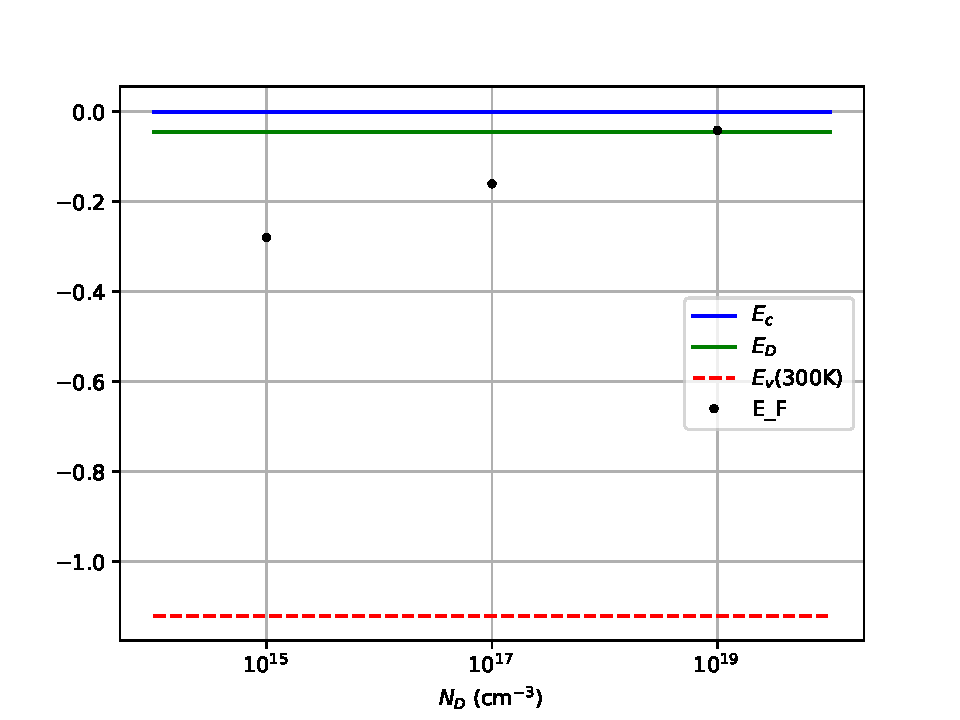
\includegraphics[width=0.9\linewidth]{Cuerpo/Ch_01/Ejercicio_01_8.pdf}
	\end{center}
